\subsection[Scenariusz - Pharming (Jakub Wyka)]{Scenariusz - Pharming}

\subsubsection[Założenia początkowe]{Założenia początkowe}
\begin{itemize}
    \item 	Raspberry Pi Zero z dostępem do internetu przez sieć wi-fi
    \item 	Przewód usb – micro usb łączący Raspberry Pi Zero z komputerem ofiary
    \item 	Raspberry Pi Zero połączone z serwerem sterującym
    \item   Pentester zalogowany w serwerze sterującym
\end{itemize}
\subsubsection[Aktorzy]{Aktorzy}
\begin{itemize}
    \item 	Pentester
    \item 	Serwer sterujący
    \item 	testowany system
    \item   Raspberry Pi Zero
\end{itemize}
\subsubsection[Opis testu]{Opis testu}
Zatruwanie DNS to metoda ataku polegająca na zmianie rekordu DNS, który 
fałszywie przypisuje nazwę domeny do adresu IP.  
Zadaniem tego ataku jest przekierowanie użytkownika na inną stronę niż ta,
 którą faktycznie chciał otworzyć. Często witryna podszywająca się wygląda 
 tak samo, przez co użytkownik nie jest świadomy ataku. Podszywanie to jest 
 nazywane phishingiem. W ten sposób użytkownik logując się do serwisu dostarcza 
 wrażliwe dane osobom przeprowadzającym atak. Połączenie DNS spoofingu z 
 zaawansowanym phishingiem nazywane jest pharmingiem.

 \subsubsection[Przebieg testu]{Przebieg testu}
Serwer sterujący służy do wydawania poleceń przez pentestera. 
Wybiera on, za pomocą którego z dostępnych urządzeń testujących 
ma zostać przeprowadzony test. Następnie wybiera rodzaj testu. W tym 
przypadku będzie to pharming. Serwer udostępni możliwość określenia
 konkretnych parametrów ataku. Dla tego typu ataku będzie to rekord DNS,
  który określi pod jaką domenę chcemy się podszyć oraz ip strony podszywającej. 
  Serwer przesyła te dane do Raspberry Pi Zero, które na tej podstawie uruchamia 
  skrypt, który jest odpowiedzialny za przeprowadzenie ataku. Do serwera odsyłany
   jest raport z wynikiem testu. 
\begin{figure}[H]
    \centering
    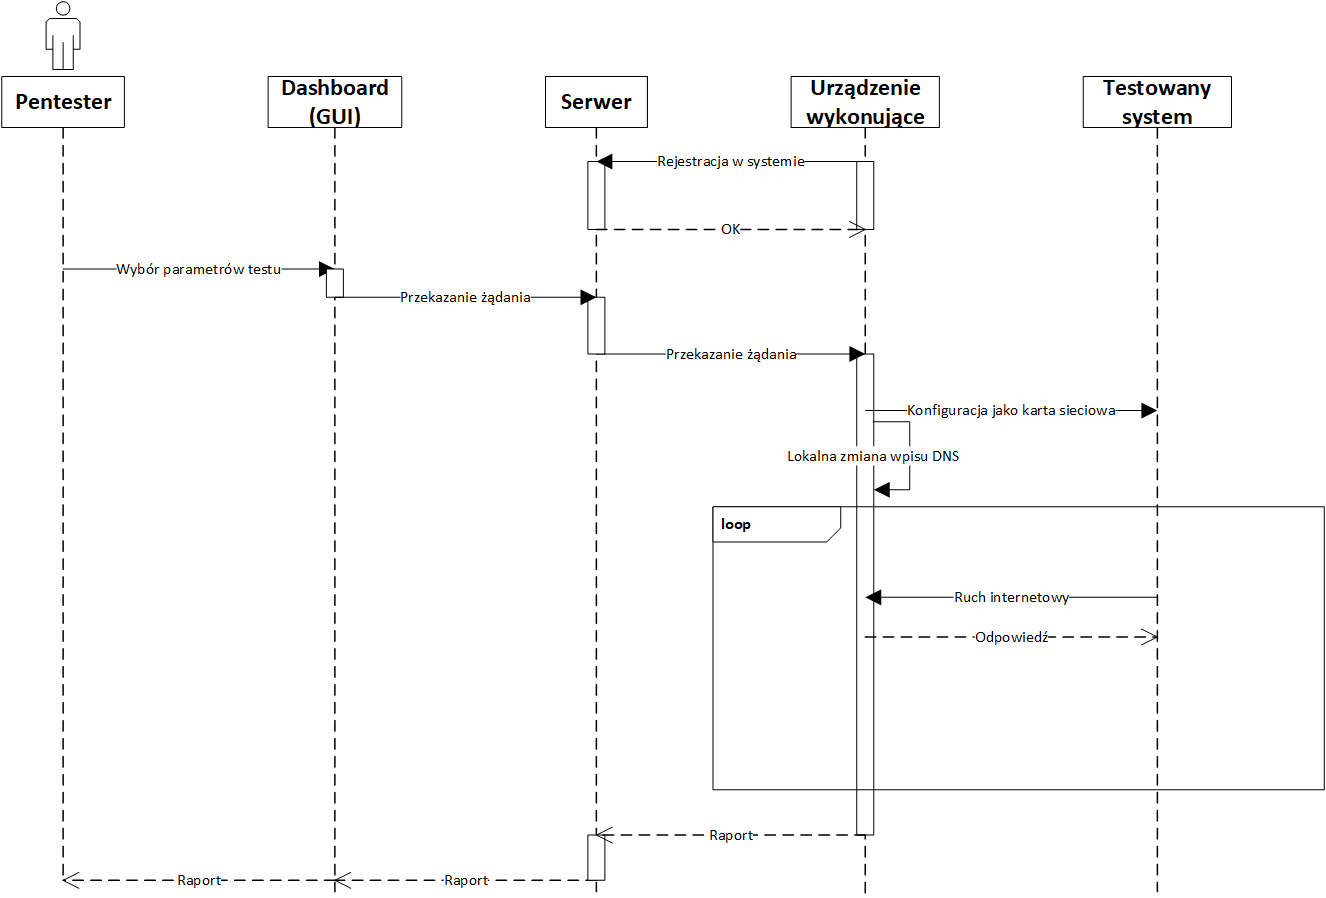
\includegraphics[width=\textwidth]{interJW}
    \caption{Diagram interakcji dla scenariusza testowego "Pharming"}
    \label{fig:pharming1}    
\end{figure}
\begin{figure}[H]
    \centering
    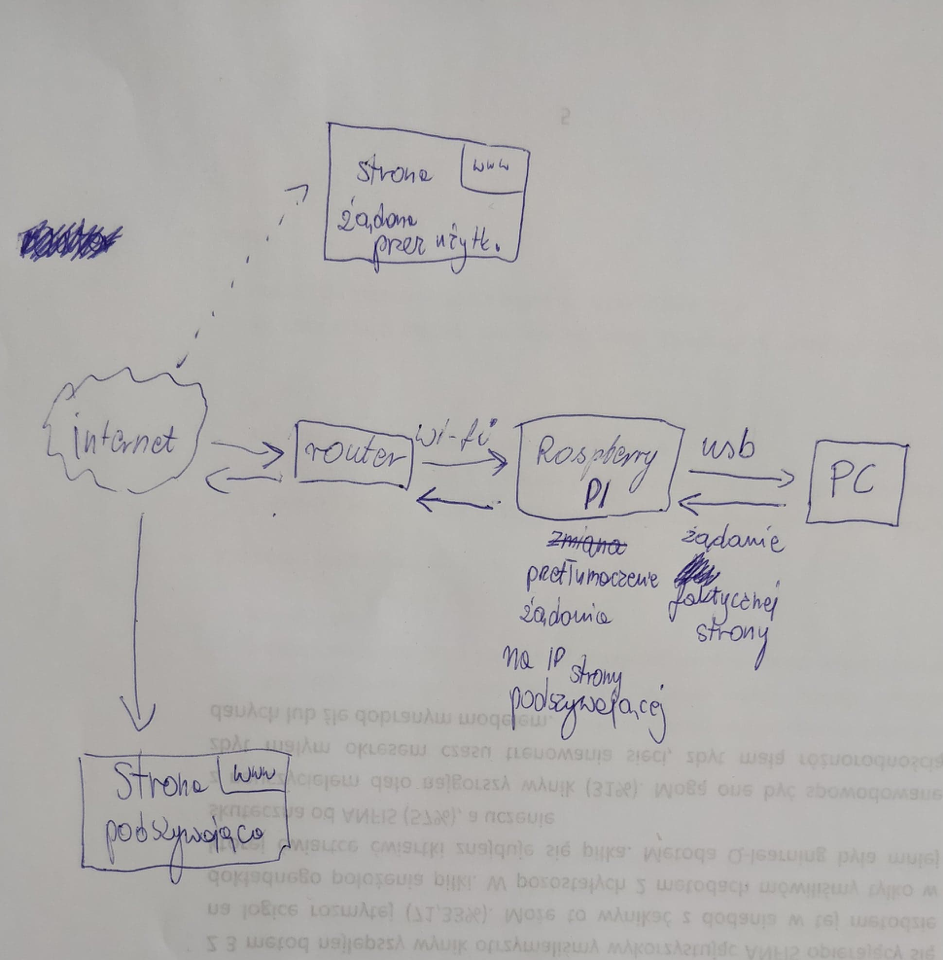
\includegraphics[width=\textwidth]{jw03}
    \caption{Pharming2}
    \label{fig:pharming2}    
\end{figure}

\subsubsection[Mozliwosc wykrycia]{Możliwość wykrycia }

Phishing jest metodą oszustwa opartą na inżynieri społecznej.
Ten scenariusz testowy ma więc na celu przetestowanie zachowania człowieka, który jest użytkownikiem systemu.
Wynika to z faktu, że jego głównym celem jest przekierowanie go na podszywającą się witrynę i
 wydobycie od niego wrażliwych danych. Należy więc zauważyć, że podmiana rekordu dns jest jedynie środkiem
 do udanego przeprowadzenia symulacji ataku phishingowego.
 Alternatywnym sposobem mogłoby być rozesłanie wiadomości drogą elektroniczą ze złośliwym hiperłączem, jednak
 atutem rozwiązania korzystającego z urządzenia USB jest możliwość przetestowania świadomości użytkowników
 na temat niebezpieczeństw jakie niosą nieznane urządzenia podłączane do systemu.

Możliwość wykrycia złośliwego urządzenia w konfiguracji karty sieciowej została opisana w sekcji ~\ref{subsec:wykrywalnoscJW},
więc w tym rozdziale opisana zostanie taka możliwość dla phishingu.
Kluczowe w dbaniu o autentyczność witryny są certyfikaty SSL. Istotny jest również ich rodzaj, gdyż wyróżniamy\cite[]{ssltypes}:
\begin{itemize}
    \item Domain Validation SSL certificates (DV) 
    \subitem Jest to najszybszy i najprostszy sposób uzyskania certyfikatu SSL. 
    \item Organization Validation (OV)
    \subitem Aby uzyskać ten certyfikat należy przejść głębszą weryfikację.
    \item Extended Validation SSL certificates (EV)
    \subitem Certyfikat zapewnia wyższy poziom zaufania i bezpieczeństwa, dzięki długiemu procesowi
    weryfikacji. Trwa ona nawet kilka tygodni, przez co jest kosztowna.
    Jednak najważniejsze jest to, że został zaprojektowany tak aby zapewniać ochronę przed
    atakami typu phishing.      
\end{itemize}

Podsumowując, użytkownicy powinni zwracać uwagę na obecność Extended Validation SSL certificate. Okazuje się,
że wbrew popularnej opinii, samo posiadanie certyfikatu ssl może nie być  wystarczające aby jednoznacznie stwierdzić bezpieczeństwo witryny.
\begin{figure}[H]
        \centering
        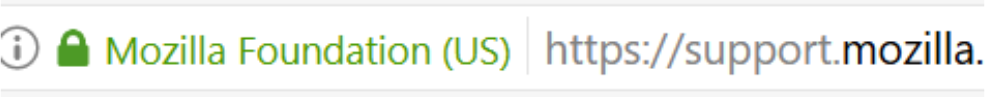
\includegraphics[width=\textwidth]{ev}
        \caption{Przykład wizualizacji posiadania certyfikatu EV przez daną witrynę, zaczerpnięty z \cite[]{sslev}}
        \label{fig:ev}
    \end{figure}